\documentclass[12pt, a4paper, simple]{eskdtext}

\usepackage{hyperref}
\usepackage{env}
\usepackage{_sty/gpi_lst}
\usepackage{_sty/gpi_toc}
\usepackage{_sty/gpi_t}
\usepackage{_sty/gpi_p}
\usepackage{_sty/gpi_u}

% Код
% \ESKDletter{О}{Л}{Р}
% \def \gpiDocTypeNum {81}
% \def \gpiDocVer {00}
% \def \gpiCode {\ESKDtheLetterI\ESKDtheLetterII\ESKDtheLetterIII.\gpiStudentGroupName\gpiStudentGroupNum.\gpiStudentCard-0\gpiDocNum~\gpiDocTypeNum~\gpiDocVer}

\def \gpiDocTopic {ОТЧЁТ ЛАБОРАТОРНОЙ РАБОТЫ №\gpiDocNum}

% Графа 1 (наименование изделия/документа)
% \ESKDcolumnI {\ESKDfontII \gpiTopic \\ \gpiDocTopic}

% Графа 2 (обозначение документа)
% \ESKDsignature {\gpiCode}

% Графа 9 (наименование или различительный индекс предприятия) задает команда
% \ESKDcolumnIX {\gpiDepartment}

% Графа 11 (фамилии лиц, подписывающих документ) задают команды
% \ESKDcolumnXIfI {\gpiStudentSurname}
% \ESKDcolumnXIfII {\gpiTeacherSurname}
% \ESKDcolumnXIfV {\gpiTeacherSurname}

\begin{document}
    \begin{ESKDtitlePage}
    \ESKDstyle{empty}
    \begin{center}
        \gpiMinEdu \\
        \gpiEdu \\
        \gpiKaf \\
    \end{center}

    \vfill

    \begin{center}
        \gpiTopic
    \end{center}

    \vfill

    \begin{center}
        \textbf{\gpiDocTopic} \\
        ПО ДИСЦИПЛИНЕ \gpiDiscipline \\
    \end{center}

    \vfill

    \begin{flushright}
        \begin{minipage}[t]{7cm}
            Выполнил:\\
            \PageTitleStudentInfo
            \PageTitleDateField
            \hspace{0pt}

            Проверил:\\
            \PageTitleTeacherInfo
            \PageTitleDateField
        \end{minipage}
    \end{flushright}

    \vfill

    \begin{center}
        \PageTitleCity~\ESKDtheYear
    \end{center}
\end{ESKDtitlePage}

    \ESKDstyle{empty}
    %
    \textbf{Цель лабораторной работы}: Разработка простого приложения, помогающего понять структуру приложения,
    освоить основные операторы, привыкнуть к среде разработки.

    Задачи лабораторной работы:
    \begin{itemize}
        \item создать новое приложение и изучить его структуру;
        \item настроить интерфейс приложения;
        \item реализовать логику приложения.
    \end{itemize}

    \subparagraph{Разработка дизайна} \hspace{0pt}

    \begin{figure}[!h]
        \centering
        \begin{minipage}{0.24\textwidth}
            \centering
            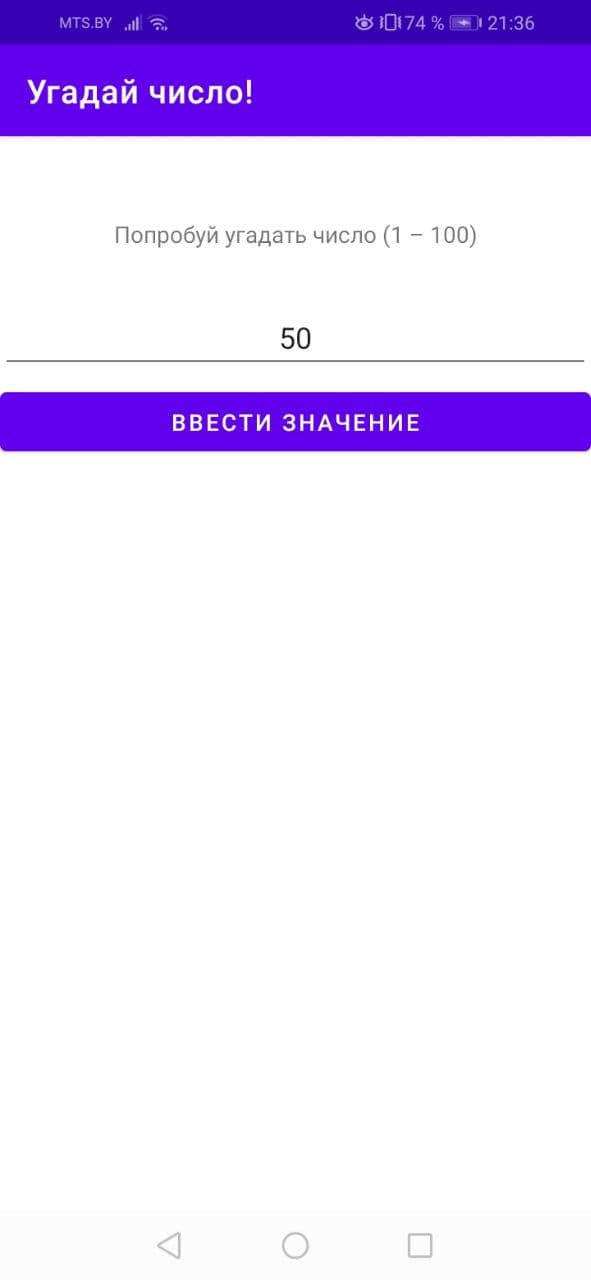
\includegraphics[width=\linewidth]
                {_assets/gpi_start.jpg}
            \caption{Старт}
            \label{fig:gpi_start}
        \end{minipage}
        \begin{minipage}{0.24\textwidth}
            \centering
            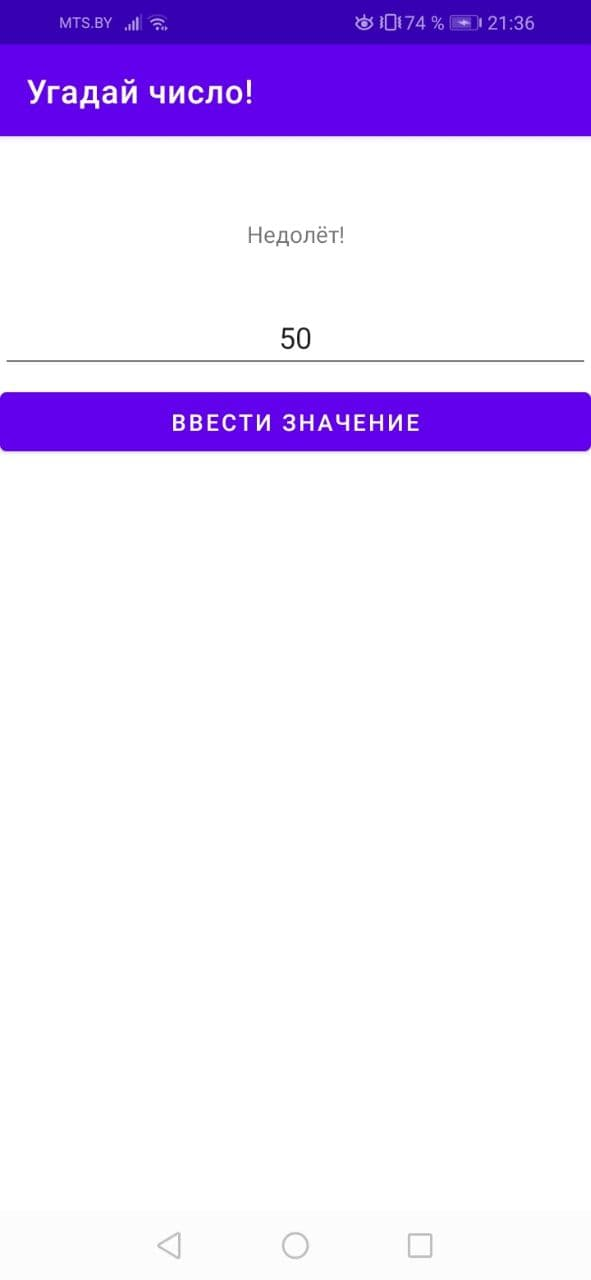
\includegraphics[width=\linewidth]
                {_assets/gpi_behind.jpg}
            \caption{Недолёт}
            \label{fig:gpi_behind}
        \end{minipage}
        \begin{minipage}{0.24\textwidth}
            \centering
            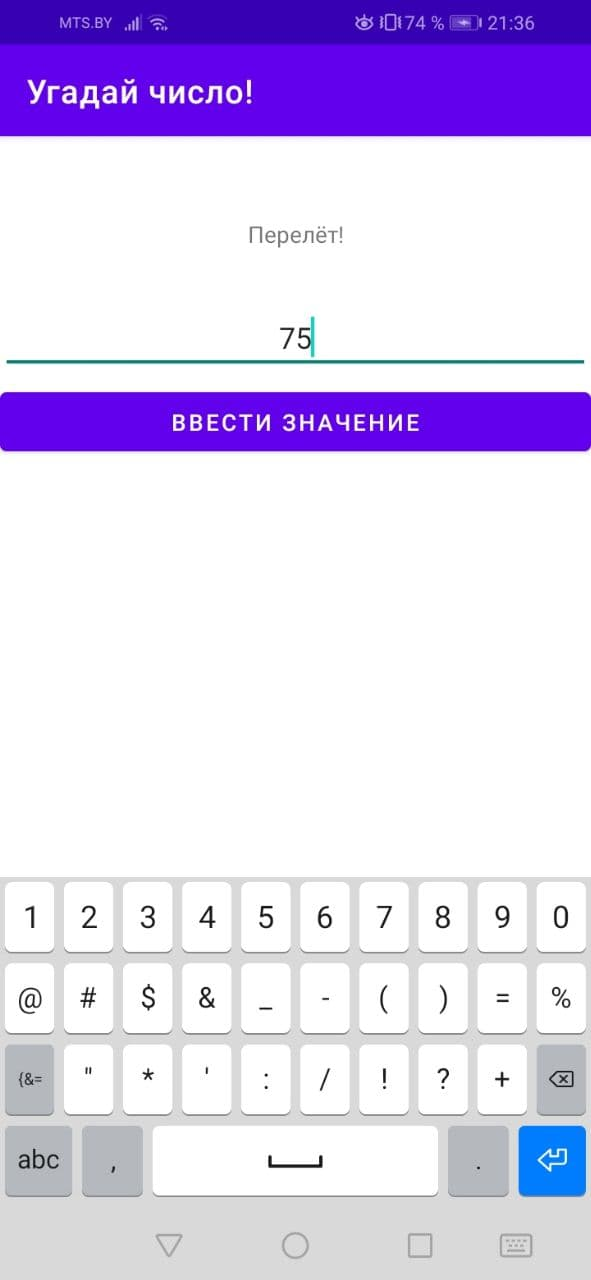
\includegraphics[width=\linewidth]
                {_assets/gpi_ahead.jpg}
            \caption{Перелёт}
            \label{fig:gpi_ahead}
        \end{minipage}
        \begin{minipage}{0.24\textwidth}
            \centering
            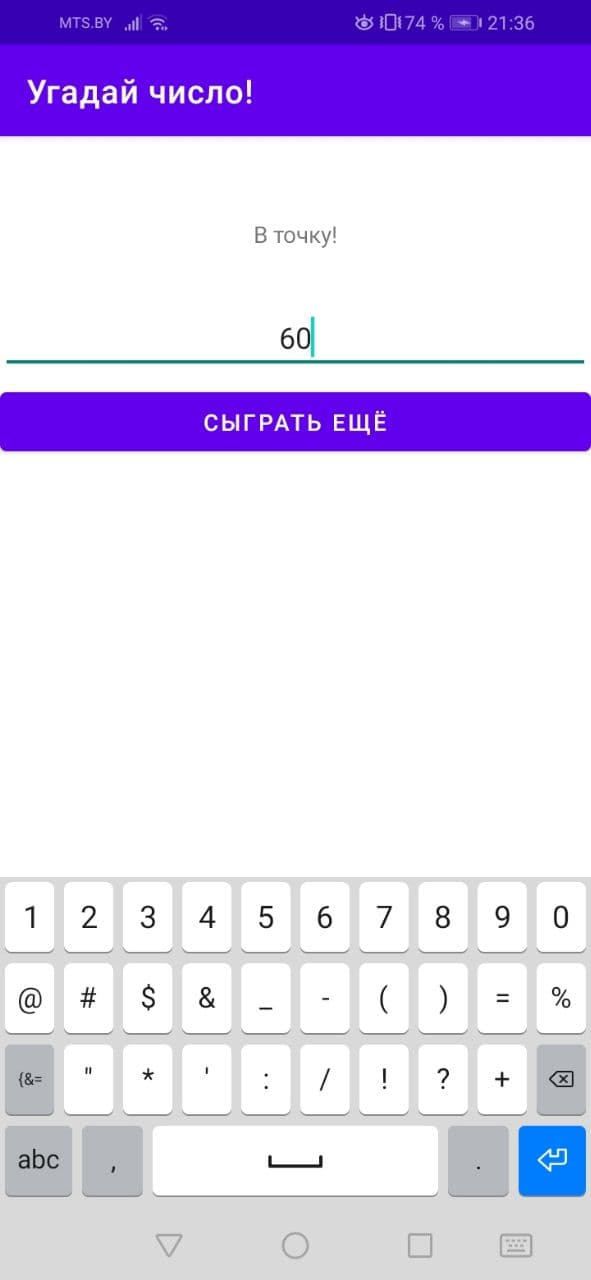
\includegraphics[width=\linewidth]
                {_assets/gpi_hit.jpg}
            \caption{В точку}
            \label{fig:gpi_hit}
        \end{minipage}
    \end{figure}

    \lstinputlisting[language=xml, name=app/src/main/res/values/strings.xml]
        {../gpi_src/gpi_rpodms6_lab2/app/src/main/res/values/strings.xml}

    \lstinputlisting[language=xml, name=app/src/main/res/layout/activity_main.xml]
        {../gpi_src/gpi_rpodms6_lab2/app/src/main/res/layout/activity_main.xml}

    \lstinputlisting[language=java, name=app/src/main/java/.../gpi_rpodms6_lab2/MainActivity.java]
        {../gpi_src/gpi_rpodms6_lab2/app/src/main/java/io/github/Pavel_Innokentevich_Galanin/gpi_rpodms6_lab2/MainActivity.java}

    \subparagraph{} \hspace{0pt}

    \textbf{Вывод}: Разработал приложение угадай число. Использовал шаблоны: TextView, EditText, Button.
    Загнал текст в файл strings.xml. Привязал функию к кнопке.

    \newpage

    \section*{Список использованных источников}
    \addcontentsline{toc}{section}{Список использованных источников}

    \begin{enumerate}
        \item[1.] Кондратюк, А. П.
        Разработка приложений для мобильных операционных систем «Android» : ЭУМК для
        студ. второй ступени (магистратуры) специальности 1-31 81 06 <<Веб-программирование и интернет-технологии>>
        физ.-мат. фак. / А.П. Кондратюк ; Брест. гос. ун-т им. А.С. Пушкина, каф. ПМиИ. – Брест : электрон. издание БрГУ, 2016. – 469 с.\\
        19.3.~Настройка интерфейса приложения cс.~275-287

        \item[2.] android layout - This view is not constrained vertically. At runtime it will jump to the left unless you add a vertical constraint - Stack Overflow
        - [Электронный ресурс]. Режим доступа:
        URL: \url{https://stackoverflow.com/questions/37859613/this-view-is-not-constrained-vertically-at-runtime-it-will-jump-to-the-left-unl}.
        (Дата обращения: 04.02.2022).
        
        \item[3.] Основы расстановки элементов интерфейса в Android Studio
        - [Электронный ресурс]. Режим доступа:
        URL: \url{https://www.youtube.com/watch?v=p3gzmkvvXkw}.
        (Дата обращения: 04.02.2022).
        
        \item[4.] android - "Missing autofillHints attribute" - Stack Overflow
        - [Электронный ресурс]. Режим доступа:
        URL: \url{https://stackoverflow.com/questions/52690296/missing-autofillhints-attribute}.
        (Дата обращения: 04.02.2022).
        
        \item[5.] OnClickListener for Multiple Buttons - Android Studio Tutorial
        URL: \url{https://www.youtube.com/watch?v=GtxVILjLcw8}.
        (Дата обращения: 04.02.2022).
        
        \item[6.] Кондратюк, А. П.
        Разработка приложений для мобильных операционных систем «Android» : ЭУМК для
        студ. второй ступени (магистратуры) специальности 1-31 81 06 <<Веб-программирование и интернет-технологии>>
        физ.-мат. фак. / А.П. Кондратюк ; Брест. гос. ун-т им. А.С. Пушкина, каф. ПМиИ. – Брест : электрон. издание БрГУ, 2016. – 469 с.\\
        §19. Лабораторная работа №2 19.7. Заключение стр 295-297
    \end{enumerate}
\end{document}
